\chapterauthor{Rami Muarrawi}
\chapter{Sensorik, I\textsuperscript{2}C-Multiplexing und Parklückenerkennung}
\label{chap:sensorik}

Eine verlässliche autonome Fahr- und Einparkfunktion setzt voraus, dass das Fahrzeug seine unmittelbare Umgebung in alle Richtungen präzise erfasst, Fehlmessungen herausfiltert und aus den Einzeldistanzen geometrisch belastbare Aussagen über freie Parklücken gewinnt. Dieses Kapitel behandelt den Aufbau des 8-fach-LiDAR-Sensorrings, die konkrete Umsetzung der \gls{xshut}-Adressvergabe unter ESP-IDF, die digitale Signalfilterung sowie die Algorithmen zur Parklücken- und Linienerkennung.

% ==============================================================================
\section{360°-Sensoranordnung und Koordinatentransformation}
\label{sec:sensor_koord}
% ==============================================================================
Um sowohl während der Vorbeifahrt an einer Parklücke als auch beim engen Rückwärts-Einparkmanöver keine toten Winkel entstehen zu lassen, wurden acht \emph{VL53L0/1XV2}-Module in einer symmetrischen \qty{45}{\degree}-Teilung rund um das Unibody-Chassis~v10.0 angeordnet (Abbildung~\ref{fig:360_fov}). Alle Sensoren liegen auf einer einheitlichen optischen Messebene ($Z_{\mathrm{Optik}} = \qty{15,0}{\milli\meter}$ über der Chassis-Unterseite bzw. \qty{13,5}{\milli\meter} Platinenmitte), wodurch Hindernisse wie Bordsteine, Begrenzungsblöcke oder benachbarte Modellfahrzeuge zuverlässig auf gleicher Höhe getroffen werden.

\begin{figure}[htbp]
  \centering
  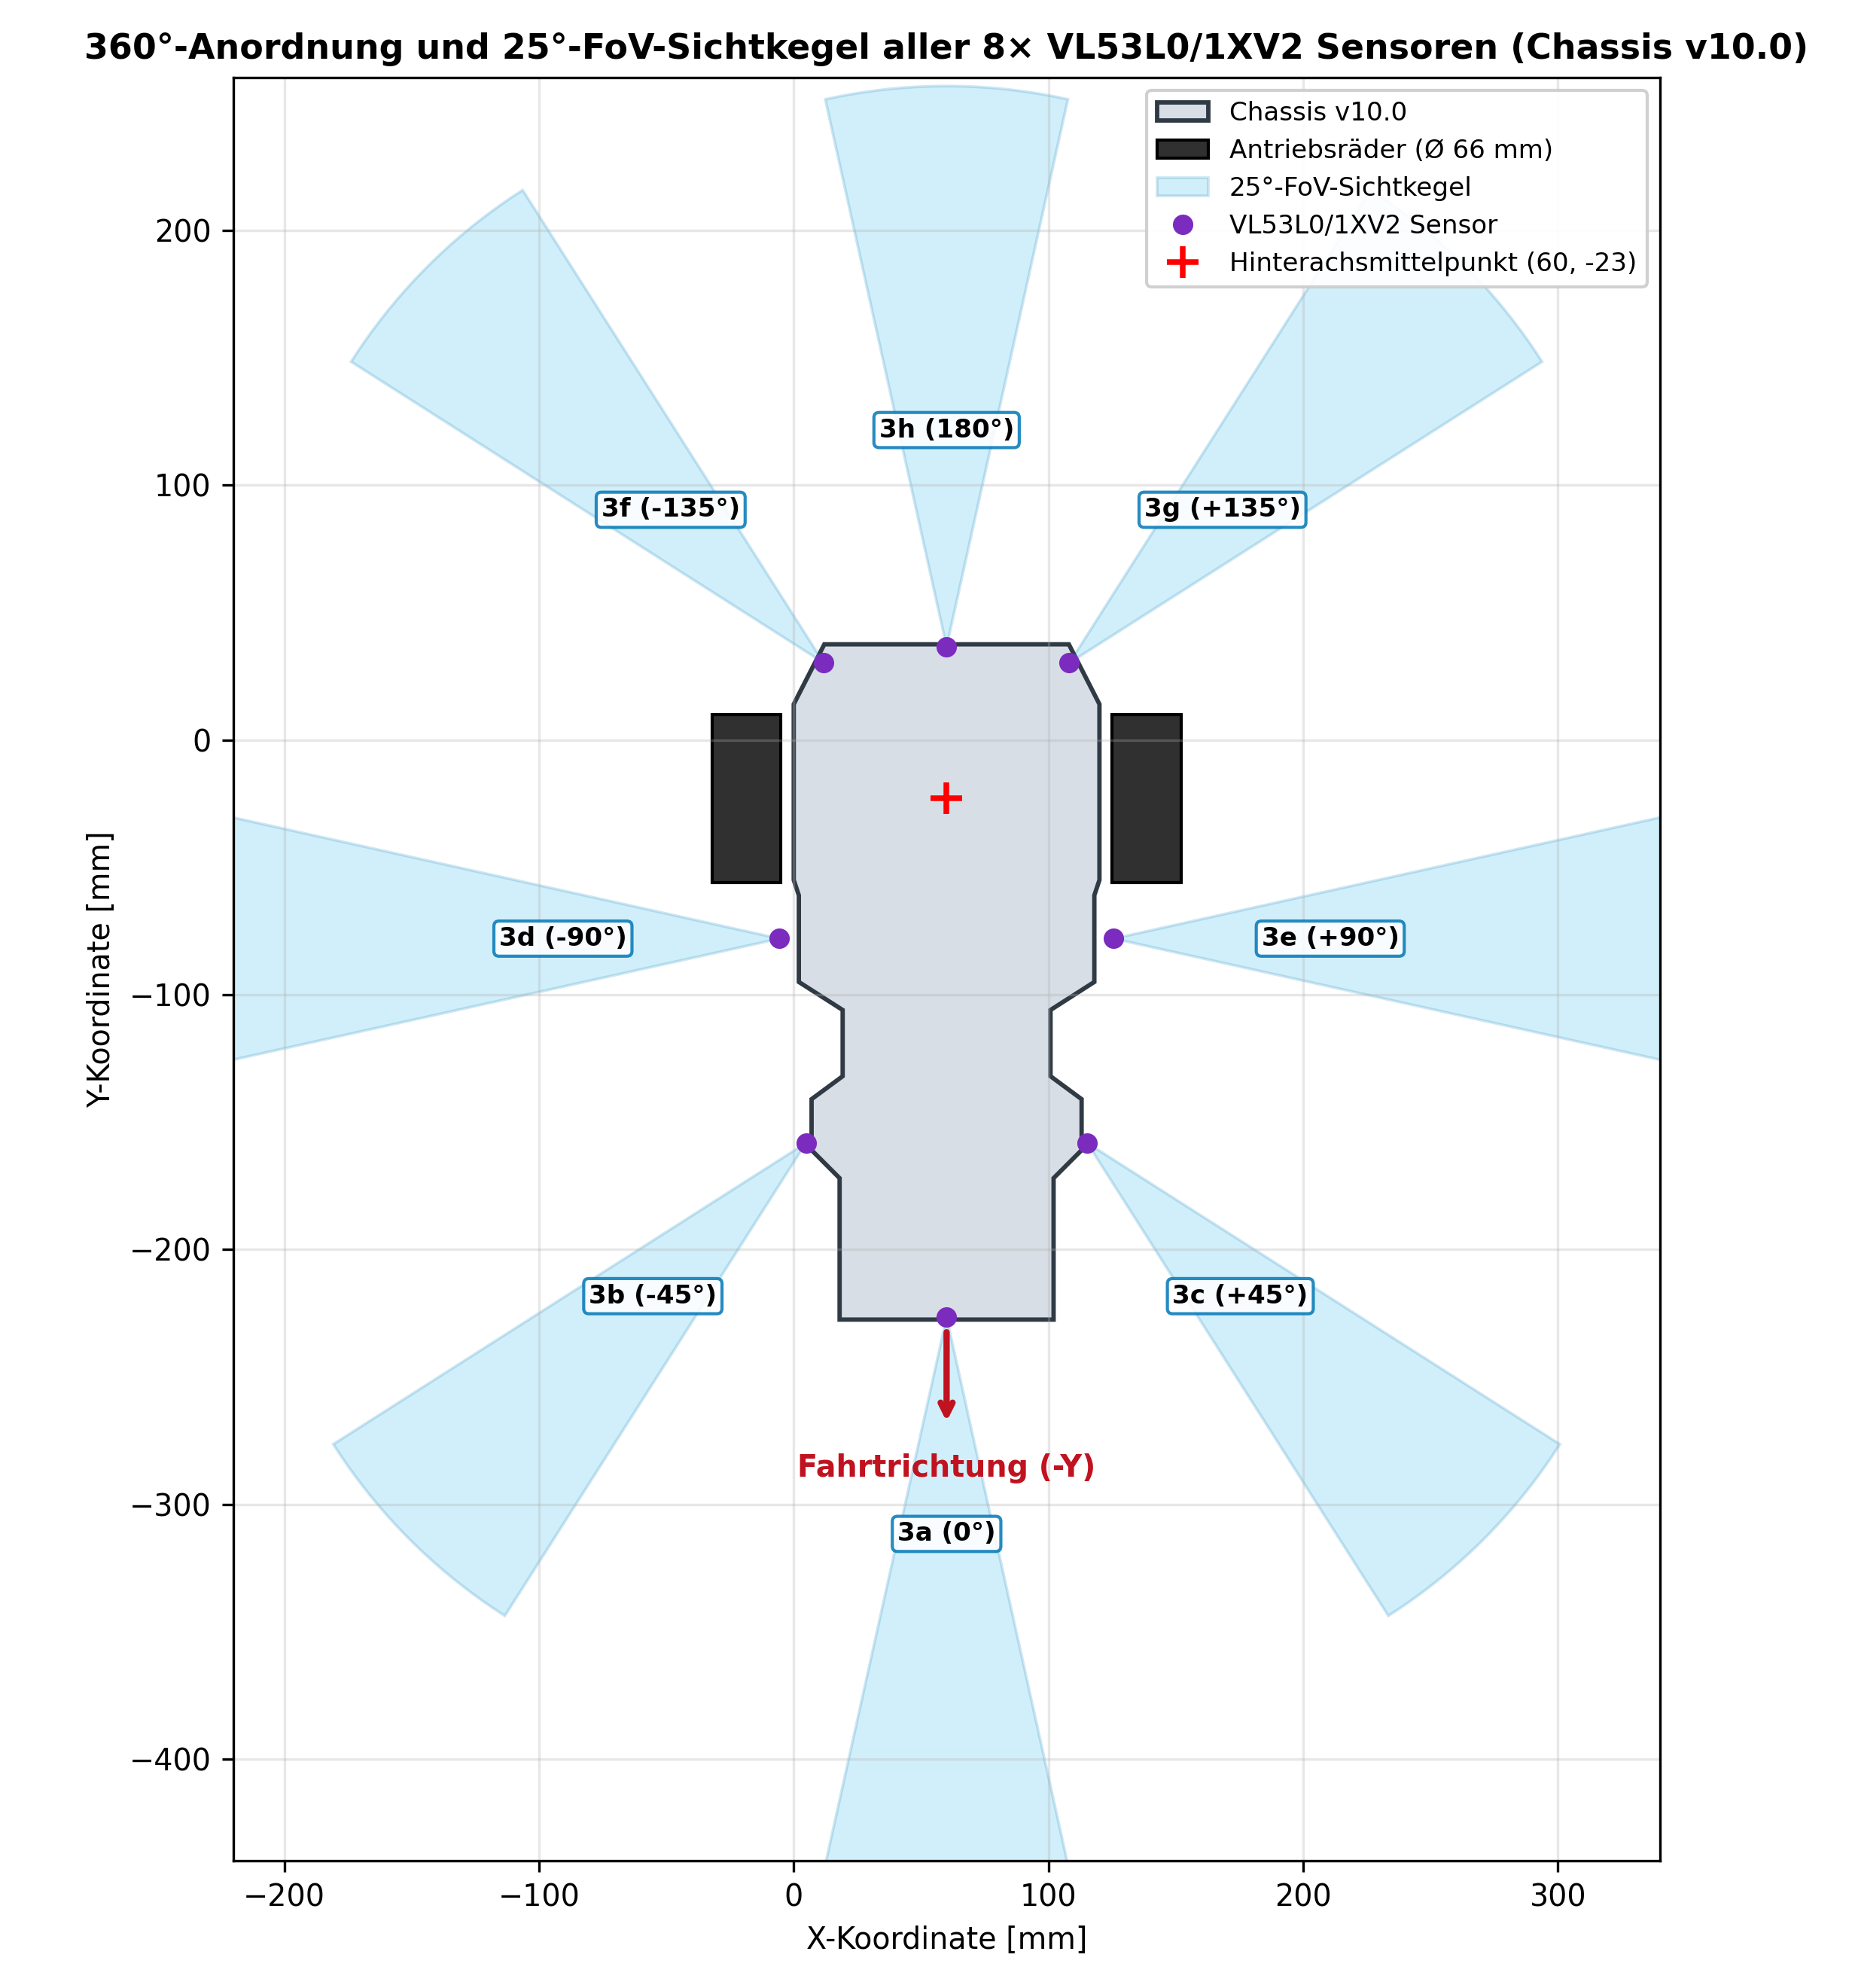
\includegraphics[width=0.78\textwidth]{figures/fig_360_fov_coverage.png}
  \caption{Geometrische Anordnung der acht \emph{VL53L0/1XV2}-Sensoren und ihrer \qty{25}{\degree}-FoV-Sichtkegel im Chassis-Koordinatensystem (Revision~v10.0).}
  \label{fig:360_fov}
\end{figure}

Tabelle~\ref{tab:lidar_koord} listet die exakten Einbaukoordinaten $(x_{s,i}, y_{s,i})$ relativ zum Chassis-Ursprung, die Ausrichtungswinkel $\psi_i$ sowie die vorgesehenen dynamischen I\textsuperscript{2}C-Adressen aller acht Sensoren auf. Der kinematische Bezugspunkt des Fahrzeugs liegt in der Mitte der Hinterachse bei $(x_{\mathrm{Achse}}, y_{\mathrm{Achse}}) = (\qty{60,0}{\milli\meter}, \qty{-23,0}{\milli\meter})$.

\begin{table}[htbp]
\centering
\caption{Geometrische Einbaupositionen, Blickwinkel und I\textsuperscript{2}C-Zieladressen der 8 LiDAR-Sensoren.}
\label{tab:lidar_koord}
\begin{tabular}{@{}l c c c c l@{}}
\toprule
\textbf{Sensor-ID} & \textbf{X [mm]} & \textbf{Y [mm]} & \textbf{Winkel $\psi_i$} & \textbf{I\textsuperscript{2}C-Adr.} & \textbf{Hauptaufgabe im Fahrbetrieb} \\
\midrule
\texttt{3a} (Front Mitte) & 60,0 & $-215,0$ & $-90^\circ$ (vorne) & \texttt{0x30} & Frontal-Hinderniswarnung \& Not-Aus \\
\texttt{3b} (Front Links) & 13,0 & $-150,0$ & $-135^\circ$ & \texttt{0x31} & Ecküberwachung beim Aus-/Einscheren links \\
\texttt{3c} (Front Rechts) & 107,0 & $-150,0$ & $-45^\circ$ & \texttt{0x32} & Vorderkanten-Bestätigung der Parklücke \\
\texttt{3d} (Seite Links) & 6,0 & $-78,0$ & $180^\circ$ & \texttt{0x33} & Linksseitige Wand-/Spurabstandsmessung \\
\texttt{3e} (Seite Rechts) & 114,0 & $-78,0$ & $0^\circ$ & \texttt{0x34} & Primärer Scanner für Längsparklücken \\
\texttt{3f} (Heck Links) & 20,0 & $+22,0$ & $+135^\circ$ & \texttt{0x35} & Ecküberwachung links beim Rückwärtsfahren \\
\texttt{3g} (Heck Rechts) & 100,0 & $+22,0$ & $+45^\circ$ & \texttt{0x36} & Hinterkanten-Abstand beim Einparken \\
\texttt{3h} (Heck Mitte) & 60,0 & $+25,0$ & $+90^\circ$ (hinten) & \texttt{0x37} & Rückwärts-Stopp vor hinterem Fahrzeug \\
\bottomrule
\end{tabular}
\end{table}

Für die Weiterverarbeitung in der Kartierung und Kollisionsprüfung wird jeder gemessene Skalarabstand $d_i$ eines Sensors $i$ in einen 2D-Hindernispunkt $(x_{H,i}, y_{H,i})$ im Fahrzeugkoordinatensystem (Ursprung Hinterachsmitte) transformiert:
\begin{equation}
  \begin{pmatrix} x_{H,i} \\ y_{H,i} \end{pmatrix}
  =
  \begin{pmatrix} x_{s,i} - x_{\mathrm{Achse}} \\ y_{s,i} - y_{\mathrm{Achse}} \end{pmatrix}
  + (d_i + d_{\mathrm{Off},i})
  \begin{pmatrix} \cos\psi_i \\ \sin\psi_i \end{pmatrix}
  \label{eq:sensor_tf}
\end{equation}
Dabei berücksichtigt $d_{\mathrm{Off},i} = \qty{11,6}{\milli\meter}$ den mechanischen Versatz zwischen dem Pod-Referenzpunkt und der realen optischen Austrittsfläche des \emph{VL53L0X}-Chips im Sensorgehäuse.

% ==============================================================================
\section{Sequenzielle XSHUT-Initialisierung und I\textsuperscript{2}C-Adressvergabe}
\label{sec:xshut_i2c}
% ==============================================================================
Alle \emph{VL53L0X}- und \emph{VL53L1X}-Sensoren starten nach dem Einschalten der Betriebsspannung werkseitig mit derselben 7-Bit-Standardadresse \texttt{0x29} \cite{ST_VL53L0X}. Würden alle acht Module gleichzeitig am gemeinsamen I\textsuperscript{2}C-Bus aktiv sein, käme es sofort zu Adresskollisionen auf der \texttt{SDA}-Leitung. Da sich die geänderte I\textsuperscript{2}C-Adresse im flüchtigen RAM des Sensors befindet, muss beim jedem Systemstart eine deterministische Initialisierungssequenz über die separaten \gls{xshut}-Steuerleitungen ablaufen (Abbildung~\ref{fig:xshut_timing}).

\begin{figure}[htbp]
  \centering
  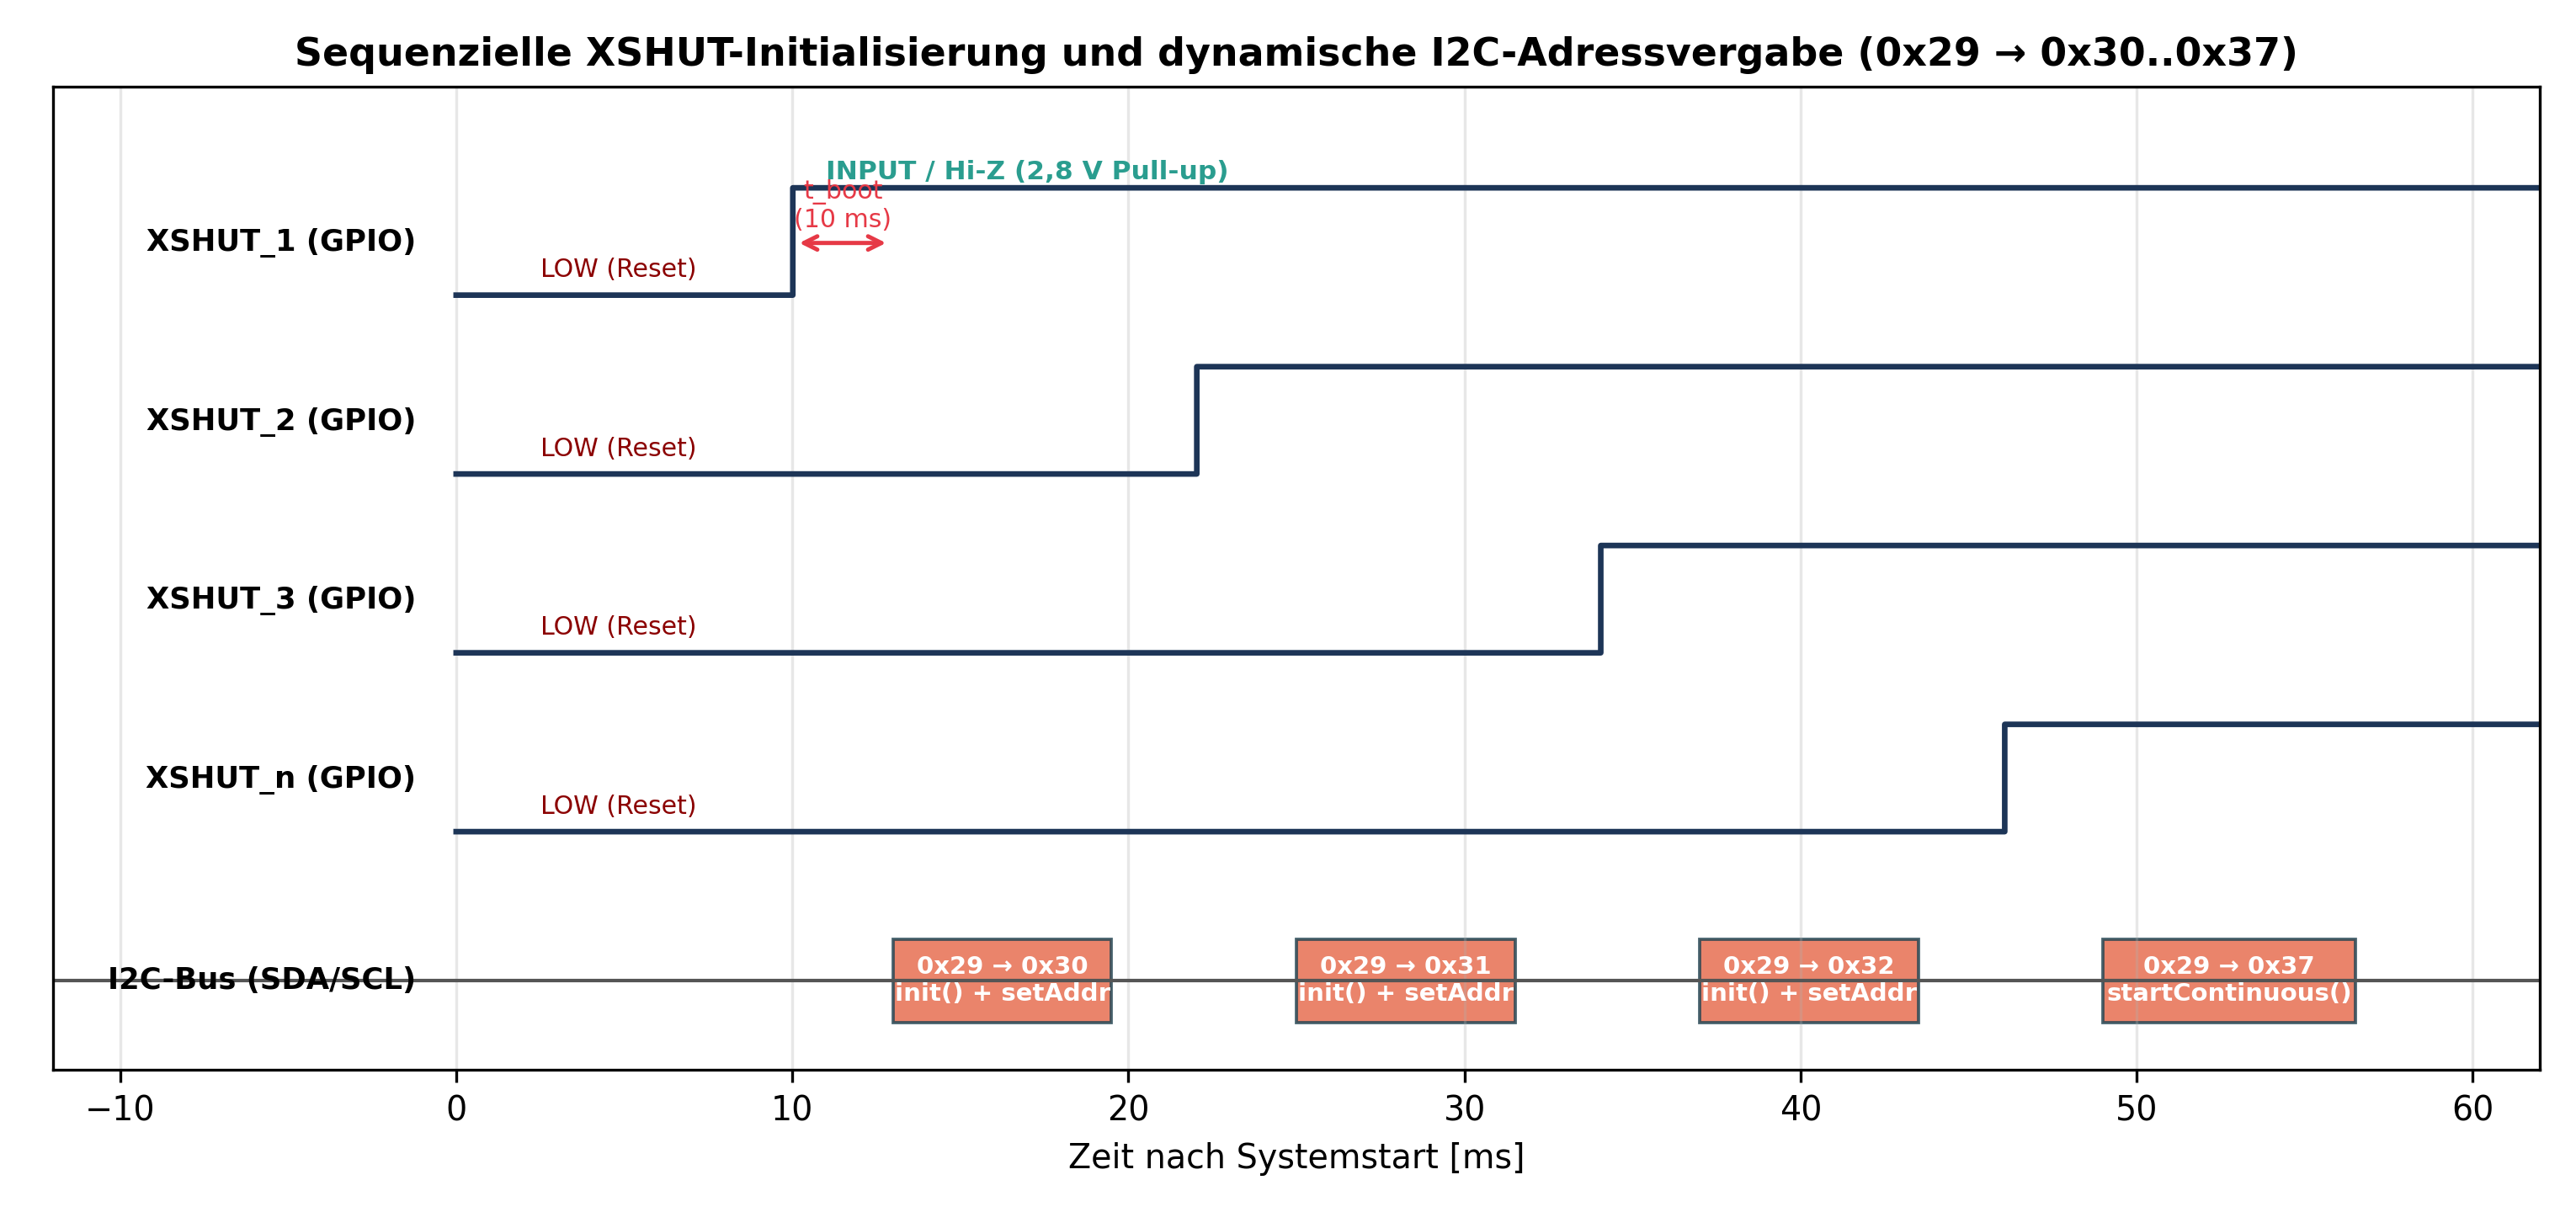
\includegraphics[width=0.96\textwidth]{figures/fig_xshut_i2c_timing.png}
  \caption{Zeitlicher Ablauf der sequenziellen XSHUT-Bootsequenz und dynamischen I\textsuperscript{2}C-Adressvergabe (\texttt{0x29} $\rightarrow$ \texttt{0x30}--\texttt{0x37}).}
  \label{fig:xshut_timing}
\end{figure}

\subsection{Elektrische Besonderheit: Hi-Z-Freigabe statt 3,3-V-High-Pegel}
Ein wichtiges Schaltungsdetail der violetten \emph{VL53L0/1XV2}-Module betrifft den Spannungspegel am \texttt{XSHUT}-Pin: Intern arbeitet der Sensor-IC mit \qty{2,8}{\volt} aus einem On-Board-LDO. Schaltet der ESP32-S3 den \texttt{XSHUT}-GPIO aktiv als \texttt{OUTPUT HIGH} auf \qty{3,3}{\volt}, fließt über die internen Schutzdioden ein unerwünschter Rückstrom in die \qty{2,8}{\volt}-Domäne. In unserer Firmware (Listing~\ref{lst:xshut_main}) wird dieses Problem sauber gelöst:
\begin{enumerate}
  \item Zu Beginn werden alle \texttt{XSHUT}-Pins als \texttt{GPIO\_MODE\_OUTPUT} auf \texttt{LOW} (\qty{0}{\volt}) gezogen, wodurch alle Sensoren sicher im Hardware-Reset verharren.
  \item Anschließend wird für jeden Sensor $i$ der zugehörige Pin auf \texttt{GPIO\_MODE\_INPUT} (hochohmig / \emph{Hi-Z}) umgeschaltet. Der auf dem Sensormodul vorhandene interne Pull-up-Widerstand zieht \texttt{XSHUT} nun exakt auf seine eigene \qty{2,8}{\volt}-Betriebsspannung.
  \item Nach einer Boot-Wartezeit von \qty{10}{\milli\second} (Datenblatt-Minimum $t_{\mathrm{boot}} = \qty{1,2}{\milli\second}$) antwortet ausschließlich Sensor $i$ auf der Default-Adresse \texttt{0x29}. Die Methode \texttt{setAddress(ADDRESSES[i])} schreibt die neue eindeutige Adresse (\texttt{0x30}, \texttt{0x31}, \dots) ins Register und startet den kontinuierlichen Messbetrieb (\texttt{startContinuous()}).
\end{enumerate}

\subsection{Reale ESP-IDF-Implementierung am Labor-Prüfstand}
Für die schrittweise Inbetriebnahme und Treibervalidierung wurde im Branch \texttt{Main\_code} (\texttt{main/main.cpp}) ein lauffähiger 4-Sensor-Prüfstand unter ESP-IDF mit portierter Pololu-C++-Bibliothek (\texttt{components/vl53l0x/VL53L0X.cpp}) aufgebaut \cite{PololuVL53L0X}. Listing~\ref{lst:xshut_main} zeigt den real getesteten Initialisierungs- und Auslesecode, der für das Gesamtfahrzeug direkt durch Erweiterung der Arrays \texttt{XSHUT\_PINS} und \texttt{ADDRESSES} auf \texttt{NUM\_SENSORS = 8} skaliert wird.

\begin{lstlisting}[language=C++,caption={Reale ESP-IDF-Implementierung der XSHUT-Initialisierung und kontinuierlichen Distanzmessung aus \texttt{main/main.cpp} (Branch \texttt{Main\_code}).},label={lst:xshut_main}]
static const int NUM_SENSORS = 4; // Gesamtfahrzeug: 8 (0x30 .. 0x37)
static const gpio_num_t XSHUT_PINS[NUM_SENSORS] = {
    GPIO_NUM_27, GPIO_NUM_26, GPIO_NUM_25, GPIO_NUM_33
};
static const uint8_t ADDRESSES[NUM_SENSORS] = {0x30, 0x31, 0x32, 0x33};

static void initI2c() {
    i2c_config_t conf = {};
    conf.mode             = I2C_MODE_MASTER;
    conf.sda_io_num       = GPIO_NUM_21;
    conf.scl_io_num       = GPIO_NUM_22;
    conf.sda_pullup_en    = GPIO_PULLUP_ENABLE;
    conf.scl_pullup_en    = GPIO_PULLUP_ENABLE;
    conf.master.clk_speed = 100000; // 100 kHz Standard-Mode
    ESP_ERROR_CHECK(i2c_param_config(I2C_NUM_0, &conf));
    ESP_ERROR_CHECK(i2c_driver_install(I2C_NUM_0, conf.mode, 0, 0, 0));
}

static void setup() {
    initI2c();
    // 1. Alle Sensoren ueber XSHUT in Hardware-Reset halten
    for (int i = 0; i < NUM_SENSORS; i++) {
        gpio_reset_pin(XSHUT_PINS[i]);
        gpio_set_direction(XSHUT_PINS[i], GPIO_MODE_OUTPUT);
        gpio_set_level(XSHUT_PINS[i], 0);
    }
    vTaskDelay(pdMS_TO_TICKS(10));

    // 2. Nacheinander via Hi-Z (INPUT) aufwecken und Adresse zuweisen
    for (int i = 0; i < NUM_SENSORS; i++) {
        gpio_set_direction(XSHUT_PINS[i], GPIO_MODE_INPUT);
        vTaskDelay(pdMS_TO_TICKS(10));
        sensors[i].setPort(I2C_NUM_0);
        sensors[i].setTimeout(500);
        if (sensors[i].init()) {
            sensors[i].setAddress(ADDRESSES[i]);
            sensors[i].startContinuous();
            sensorOk[i] = true;
        }
    }
}
\end{lstlisting}

\subsection{I\textsuperscript{2}C-Zeitbudget-Analyse für den 8-Sensor-Betrieb}
\label{sec:i2c_zeitbudget}
Da alle acht \emph{VL53L0X}-Sensoren sowie die \emph{LSM6DSV}-IMU denselben I\textsuperscript{2}C-Bus nutzen, muss rechnerisch geprüft werden, ob das serielle Auslesen innerhalb der \qty{40}{\milli\second}-Periode des \texttt{LidarImuTask} zuverlässig gelingt. Im kontinuierlichen Messbetrieb (\texttt{startContinuous()}) ermittelt jeder Sensor seine Distanz autonom im Hintergrund. Das Auslesen eines 16-Bit-Ergebnisregisters (\texttt{RESULT\_RANGE\_STATUS + 10}) samt Status-Abfrage und Interrupt-Quittierung umfasst rund 6~Byte pro Sensor (inkl. Start-, Adress-, Register- und Stopp-Bits ca. 60~Taktzyklen). Für alle acht Sensoren ergibt sich damit eine reine Busbelegungszeit von:
\begin{align}
  t_{\mathrm{Bus,100k}} &= 8 \cdot \frac{60}{\qty{100}{\kilo\hertz}} = \qty{4,80}{\milli\second} \quad (\text{12\,\% Buslast bei }\qty{40}{\milli\second}\text{ Zyklus}) \label{eq:i2c_t100} \\
  t_{\mathrm{Bus,400k}} &= 8 \cdot \frac{60}{\qty{400}{\kilo\hertz}} = \qty{1,20}{\milli\second} \quad (\text{3\,\% Buslast bei }\qty{40}{\milli\second}\text{ Zyklus}) \label{eq:i2c_t400}
\end{align}
Selbst im konservativen \qty{100}{\kilo\hertz}-Standard-Mode verbleiben über \qty{34}{\milli\second} Reserve pro Zyklus für die IMU-Abfrage und die digitale Filterung.

% ==============================================================================
\section{Messwertvorverarbeitung und digitale Filterung}
\label{sec:filterung}
% ==============================================================================
Rohdaten von \gls{tof}-Sensoren enthalten im praktischen Laborbetrieb zwei typische Störungsarten: erstens sporadische Ausreißer (\emph{Spikes}) durch Spiegelreflexionen oder ungültige Messungen (\texttt{d >= 8190} bzw. \texttt{timeoutOccurred()}), und zweitens statistisches Messrauschen im Bereich von $\pm \qtyrange{3}{8}{\milli\meter}$. Würden ungefilterte Rohwerte direkt in die Flankenerkennung der Parklückensuche eingespeist, könnte ein einziger Fehlimpuls das vorzeitige Ende einer Parklücke vortäuschen.

Aus diesem Grund durchläuft jeder Sensorkanal eine zweistufige Filterkette:
\begin{enumerate}
  \item \textbf{Plausibilitätsprüfung und 3-Punkte-Medianfilter:} Werte außerhalb des gültigen Messbereichs ($d < \qty{20}{\milli\meter}$ oder $d \ge \qty{8190}{\milli\meter}$) werden auf den Maximalwert $d_{\max} = \qty{1500}{\milli\meter}$ (freier Raum) geklemmt bzw. bei Timeout als ungültig markiert. Der anschließende Medianfilter über die letzten drei Messwerte
  \begin{equation}
    d_{\mathrm{med}}[k] = \mathrm{median}\bigl(d_{\mathrm{roh}}[k],\, d_{\mathrm{roh}}[k-1],\, d_{\mathrm{roh}}[k-2]\bigr)
    \label{eq:median}
  \end{equation}
  eliminiert einzelne Ausreißer vollständig, ohne echte Kantenübergänge (wie den Beginn einer Parklücke) zu verschmieren.
  \item \textbf{Exponentiell gewichteter gleitender Mittelwert (\gls{ema}):} Zur Glättung des verbleibenden Grundrauschens folgt ein rekursiver Tiefpass erster Ordnung:
  \begin{equation}
    d_{\mathrm{filt}}[k] = \alpha \cdot d_{\mathrm{med}}[k] + (1 - \alpha) \cdot d_{\mathrm{filt}}[k-1], \qquad \alpha \in (0, 1]
    \label{eq:ema}
  \end{equation}
  Mit $\alpha = 0{,}35$ bei einer Messrate von \qty{25}{\hertz} ($T_{\mathrm{LiDAR}} = \qty{40}{\milli\second}$) ergibt sich eine effektive Filterzeitkonstante von ca. \qty{95}{\milli\second} -- schnell genug für scharfe Parklückenkanten bei einer Suchgeschwindigkeit von $v_{\mathrm{Scan}} = \qty{0,25}{\meter\per\second}$ (entspricht \qty{24}{\milli\meter} Wegstrecke), aber ruhig genug für eine stabile Abstandsregelung.
\end{enumerate}

% ==============================================================================
\section{Geometrische Parklückenerkennung}
\label{sec:parkluecke}
% ==============================================================================
Die Erkennung einer geeigneten Längsparklücke auf der rechten Fahrzeugseite basiert auf der zeitlichen Kopplung des seitlichen LiDAR-Sensors \texttt{3e} ($0^\circ$, rechts) mit der zurückgelegten Wegstrecke $s(t)$ aus der Hinterachs-Odometrie (Abbildung~\ref{fig:parking_geom}).

\begin{figure}[htbp]
  \centering
  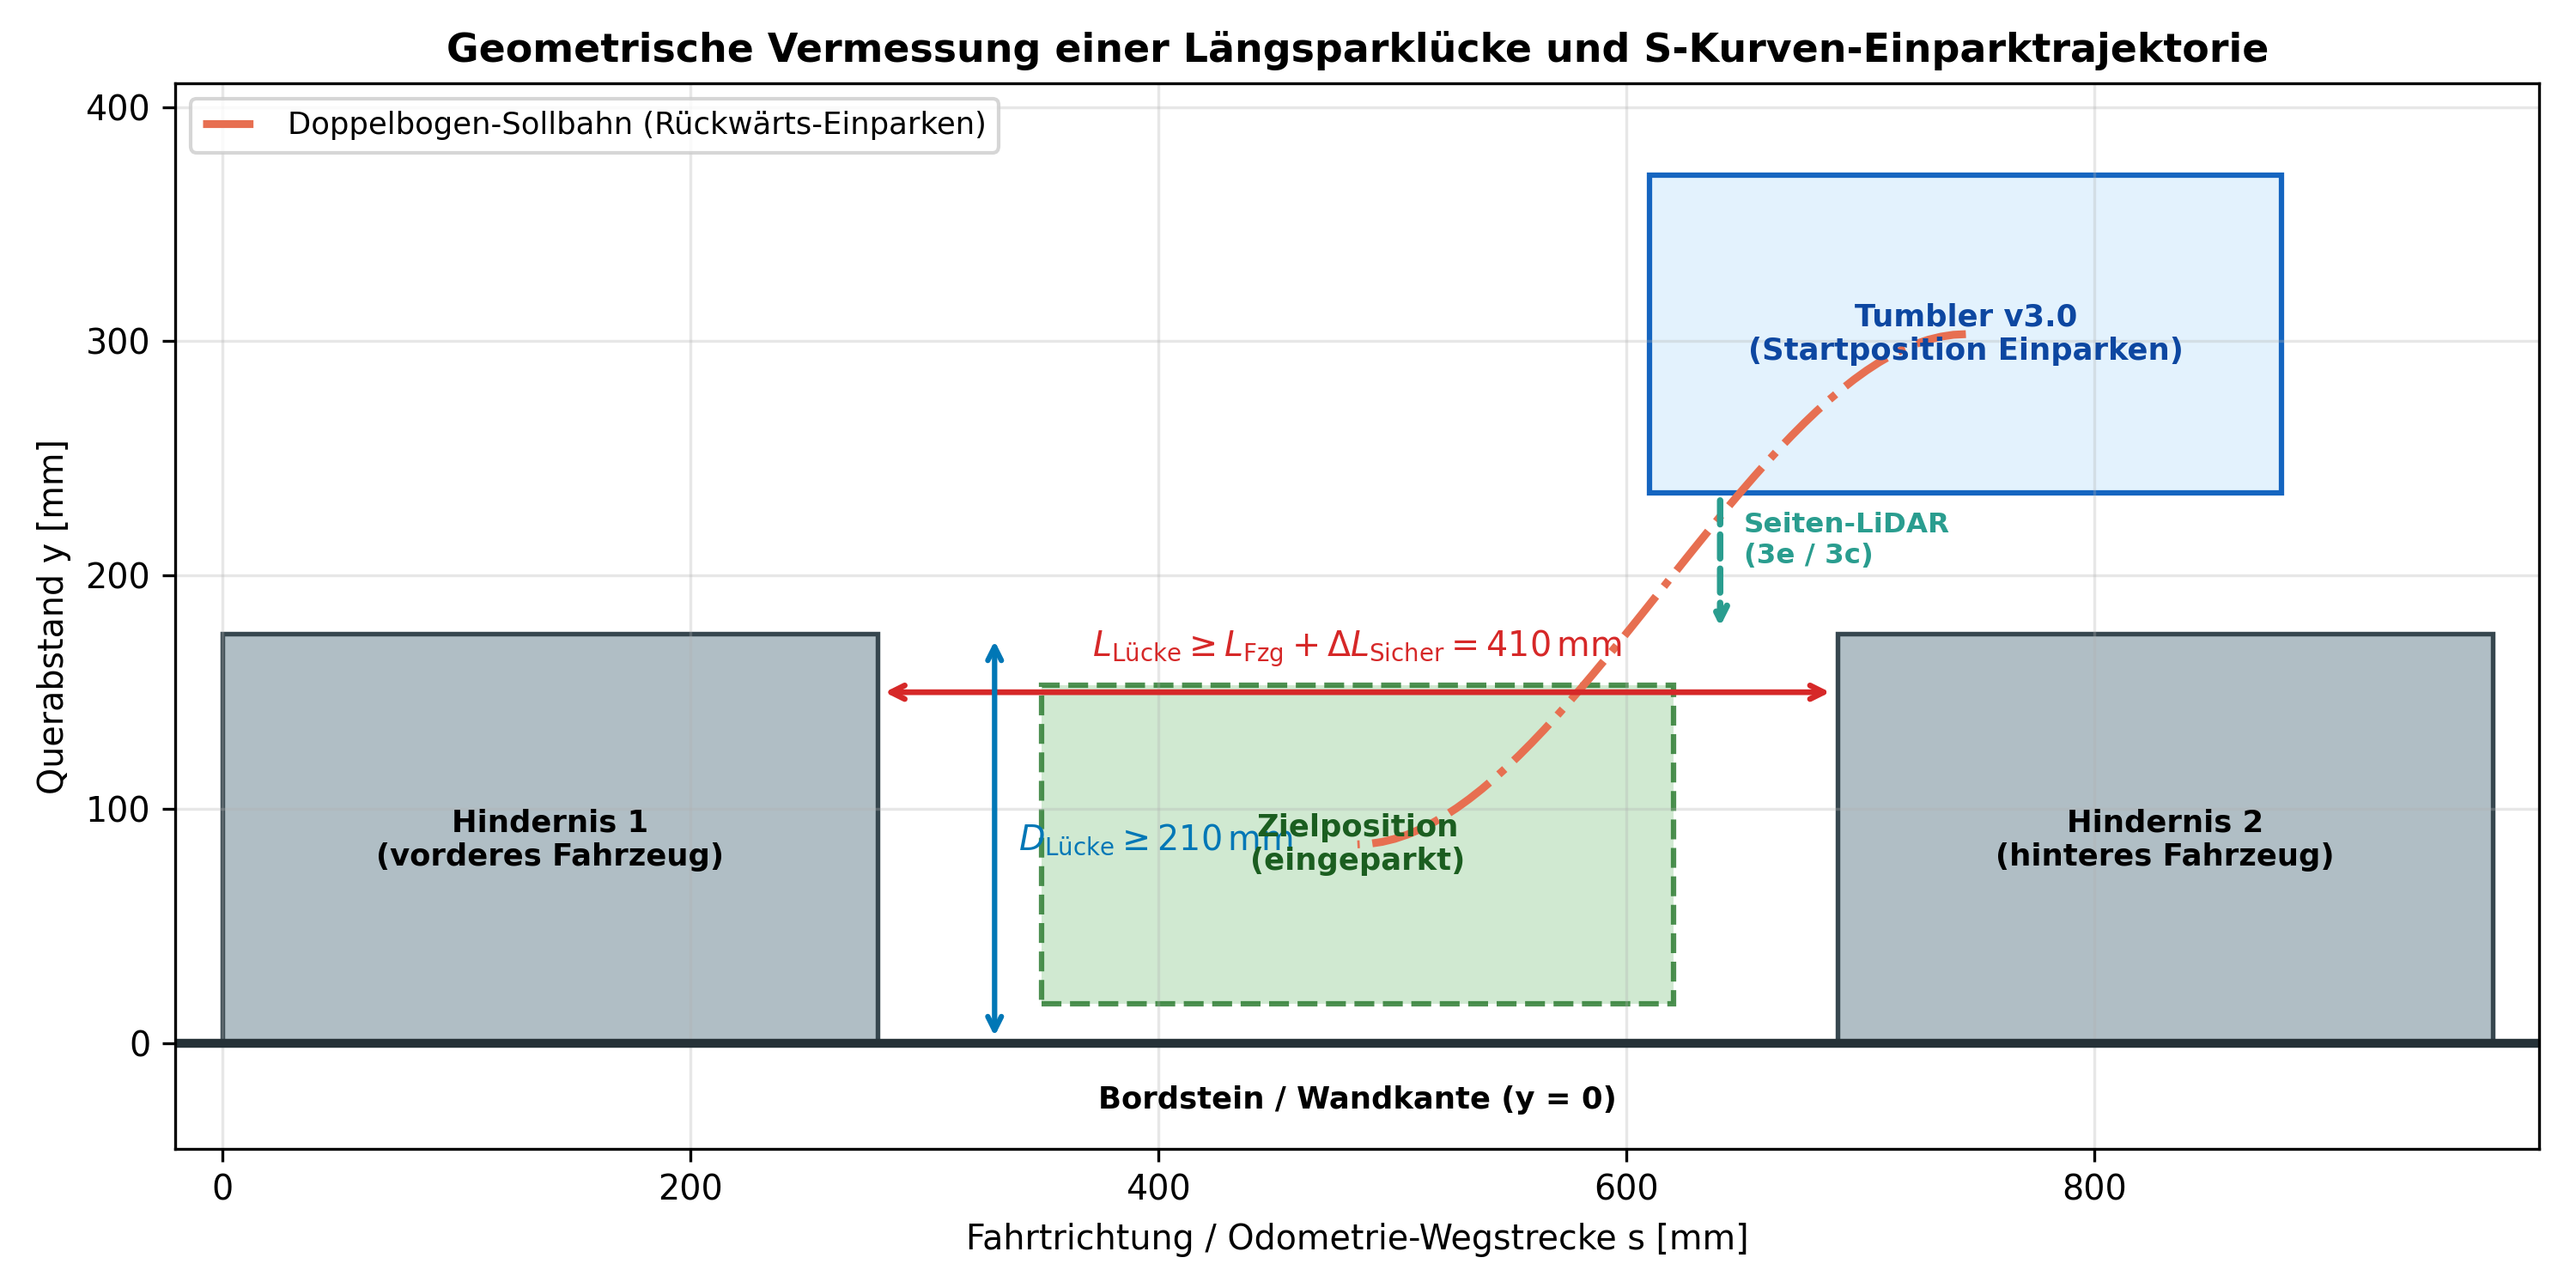
\includegraphics[width=0.98\textwidth]{figures/fig_parking_geometry.png}
  \caption{Geometrische Vermessung einer Längsparklücke über Seiten-LiDAR (\texttt{3e}) und Odometrie-Wegstrecke $s$ sowie Solltrajektorie für das Rückwärts-Einparken.}
  \label{fig:parking_geom}
\end{figure}

\subsection{Kriterien für eine befahrbare Längsparklücke}
Das Fahrzeug besitzt in Revision~v10.0 eine Gesamtlänge von $L_{\mathrm{Fzg}} = \qty{270,4}{\milli\meter}$ und eine Breite über die Antriebsräder von $B_{\mathrm{Fzg}} = \qty{184,0}{\milli\meter}$. Damit ein sicheres Rückwärts-Einparken ohne Touchieren der begrenzenden Hindernisse möglich ist, muss eine erkannte Lücke zwei geometrische Bedingungen gleichzeitig erfüllen:
\begin{align}
  L_{\mathrm{L\ddot{u}cke}} &= s_{\mathrm{Ende}} - s_{\mathrm{Start}} \ge L_{\mathrm{Fzg}} + \Delta L_{\mathrm{Sicher}} = \qty{270,4}{\milli\meter} + \qty{139,6}{\milli\meter} = \qty{410}{\milli\meter} \label{eq:gap_len} \\
  D_{\mathrm{L\ddot{u}cke}} &= d_{\mathrm{3e,min,L\ddot{u}cke}} - d_{\mathrm{Wand,ref}} \ge B_{\mathrm{Fzg}} + \Delta B_{\mathrm{Sicher}} = \qty{184,0}{\milli\meter} + \qty{26,0}{\milli\meter} = \qty{210}{\milli\meter} \label{eq:gap_depth}
\end{align}
Um Flattern an der Hinderniskante zu vermeiden, arbeitet die Kanten-Erkennung mit einer Hysterese:
\begin{itemize}
  \item \textbf{Eintritt in mögliche Lücke (\emph{Rising Edge}):} Wenn $d_{\mathrm{3e,filt}} > d_{\mathrm{Wand,ref}} + \qty{180}{\milli\meter}$, wird der aktuelle Odometriestand als $s_{\mathrm{Start}}$ gespeichert und die minimale gemessene Lückentiefe $D_{\mathrm{min}}$ laufend mitgeführt.
  \item \textbf{Ende der Lücke (\emph{Falling Edge}):} Fällt $d_{\mathrm{3e,filt}}$ wieder unter $d_{\mathrm{Wand,ref}} + \qty{120}{\milli\meter}$, wird $s_{\mathrm{Ende}}$ gespeichert. Sind beide Bedingungen \eqref{eq:gap_len} und \eqref{eq:gap_depth} erfüllt, meldet das Sensorik-Modul eine gültige Parklücke an die Einpark-FSM (Kapitel~\ref{sec:einpark_fsm}).
\end{itemize}

\begin{lstlisting}[language=C++,caption={Zweistufiger Median-3- und EMA-Distanzfilter sowie Hysterese-Parklückendetektor (C++).},label={lst:gap_filter}]
struct LidarFilter {
    uint16_t ring[3] = {1500, 1500, 1500};
    uint8_t  idx     = 0;
    float    ema     = 1500.0f;

    float update(uint16_t rawMm, bool timeout) {
        uint16_t clamped = (timeout || rawMm >= 8190 || rawMm < 20) ? 1500 : rawMm;
        ring[idx] = clamped;
        idx = (idx + 1) % 3;
        // 3-Punkte-Median ohne dynamische Speicherallokation
        uint16_t a = ring[0], b = ring[1], c = ring[2];
        uint16_t med = (a > b) ? ((b > c) ? b : ((a > c) ? c : a))
                               : ((a > c) ? a : ((b > c) ? c : b));
        ema = 0.35f * static_cast<float>(med) + 0.65f * ema;
        return ema;
    }
};

struct GapDetector {
    bool  inGap    = false;
    float sStartMm = 0.0f;
    float minDepth = 1500.0f;
    float wallRef  = 140.0f; // Referenzabstand zur geparkten Fahrzeugreihe

    bool update(float dRightMm, float odoSMm, float &foundLenMm) {
        if (!inGap && dRightMm > wallRef + 180.0f) {
            inGap = true;
            sStartMm = odoSMm;
            minDepth = dRightMm - wallRef;
        } else if (inGap) {
            float curDepth = dRightMm - wallRef;
            if (curDepth < minDepth) minDepth = curDepth;
            if (dRightMm < wallRef + 120.0f) {
                inGap = false;
                float len = odoSMm - sStartMm;
                if (len >= 410.0f && minDepth >= 210.0f) {
                    foundLenMm = len;
                    return true; // Gueltige Laengsparkluecke bestaetigt!
                }
            }
        }
        return false;
    }
};
\end{lstlisting}

% ==============================================================================
\section{Optische Linienerkennung und Kalibrierung}
\label{sec:linienerkennung}
% ==============================================================================
Für die Spurführung während der Anfahrt werden die sechs analogen Kanäle \texttt{LS1}--\texttt{LS6} der Liniensensor-Platine (Kapitel~\ref{sec:liniensensor_pcb}) über \texttt{ADC1\_CH3} bis \texttt{ADC1\_CH9} mit \qty{100}{\hertz} abgetastet. Da Umgebungslicht, Bodenreflexion und Bauteiltoleranzen der einzelnen \emph{CNY70} variieren, durchläuft das Fahrzeug vor der Fahrt eine Zweipunkt-Kalibrierung über der hellen Fahrbahn ($U_{\mathrm{wei\ss},i}$) und der schwarzen Linie ($U_{\mathrm{schwarz},i}$).

Jeder Rohmesswert $U_i$ wird anschließend auf einen normierten Schwärzungsgrad $n_i \in [0, 1]$ abgebildet (wobei $n_i = 1$ einer dunklen Linie entspricht, da $U_{\mathrm{schwarz},i} > U_{\mathrm{wei\ss},i}$):
\begin{equation}
  n_i = \mathrm{clamp}_{[0, 1]}\!\left(\frac{U_i - U_{\mathrm{wei\ss},i}}{U_{\mathrm{schwarz},i} - U_{\mathrm{wei\ss},i}}\right)
  \label{eq:ls_norm}
\end{equation}
Mit den realen mechanischen Sensorpositionen $x_i \in \{-25, -15, -5, +5, +15, +25\}\,\mathrm{mm}$ (\qty{10}{\milli\meter}-Raster symmetrisch zur Fahrzeuglängsachse) ergibt sich die stufenlose seitliche Linienablage $e_{\mathrm{Linie}}$ in Millimetern durch gewichtete Schwerpunktberechnung:
\begin{equation}
  e_{\mathrm{Linie}} = \frac{\sum_{i=1}^{6} x_i \cdot n_i}{\sum_{i=1}^{6} n_i}, \qquad \text{für } \sum_{i=1}^{6} n_i > \varepsilon_{\min}
  \label{eq:ls_centroid}
\end{equation}
Unterschreitet die Summe $\sum n_i$ den Schwellwert $\varepsilon_{\min} = 0{,}35$, erkennt die Firmware einen Linienverlust und hält entweder die letzte bekannte Suchrichtung oder schaltet sicher in den Stoppzustand. Umgekehrt signalisiert $\sum n_i > 4{,}8$ eine querliegende Stopp- oder Startmarkierung auf dem Testparcours.
